\documentclass[12pt]{article}

\usepackage{sbc-template}

\usepackage{graphicx,url}

\usepackage[brazil]{babel}   
\usepackage[latin1]{inputenc}
\usepackage[T1]{fontenc}

\usepackage{listings}
\usepackage{xcolor}

\lstdefinestyle{customc++}{
  belowcaptionskip=1\baselineskip,
  breaklines=true,
  frame=L,
  xleftmargin=\parindent,
  language=C++,
  showstringspaces=false,
  basicstyle=\footnotesize\ttfamily,
  keywordstyle=\bfseries\color{green!40!black},
  commentstyle=\itshape\color{red!70!black},
  %identifierstyle=\color{blue},
  stringstyle=\color{orange},
}
     
\sloppy

\title{TODO: Title}

\author{Matheus B. Nascimento\inst{1},
		Wisllay Vitrio\inst{1}
}

\address{
	Instituto de Inform�tica -- Universidade Federal de Goi�s (UFG)\\
	Caixa Postal 131 -- CEP 74.001-970 -- Goi�nia -- GO -- Brasil
}

\begin{document} 

\maketitle

\begin{abstract}
Abstract. Abstract. Abstract. Abstract. Abstract. Abstract. Abstract. Abstract. Abstract. Abstract.
\end{abstract}
     
\begin{resumo}
Resumo. Resumo. Resumo. Resumo. Resumo. Resumo. Resumo. Resumo. Resumo. Resumo. Resumo. Resumo.
\end{resumo}

\section{Introdu��o}
\label{sec:introducao}

Introdu��o

\section{Proposta}
\label{sec:proposta}

Proposta

\section{Implementa��o}
\label{sec:implementacao}

Implementa��o

\begin{lstlisting}[style=customc++]
// Stops retransmission attempts on remote station manager (RTS/CTS and Data)
Config::SetDefault("ns3::WifiRemoteStationManager::MaxSsrc",UintegerValue(0));
Config::SetDefault("ns3::WifiRemoteStationManager::MaxSlrc",UintegerValue(0));
\end{lstlisting}


\begin{lstlisting}[style=customc++]
// Create default PHY and Channel
YansWifiChannelHelper chan = YansWifiChannelHelper::Default();
YansWifiPhyHelper phy = YansWifiPhyHelper::Default();
// Set channel
phy.SetChannel(chan.Create());
\end{lstlisting}

\begin{lstlisting}[style=customc++]
// Set Reception Gain to 0
phy.Set("RxGain", DoubleValue(0));
// Disable signal detection so the sending devices don't backoff
phy.Set("EnergyDetectionThreshold", DoubleValue(0));
// Stop the PHY layer from declaring 'CCA_BUSY'
phy.Set("CcaMode1Threshold", DoubleValue(0));
\end{lstlisting}


\begin{lstlisting}[style=customc++]
// Create and setup mobility
MobilityHelper mob;
mob.SetPositionAllocator("ns3::GridPositionAllocator",
	"MinX", DoubleValue(0),
	"MinY", DoubleValue(0),
	"DeltaX", DoubleValue(gridDeltaX),
	"DeltaY", DoubleValue(gridDeltaY),
	"GridWidth", UintegerValue(gridWidth),
	"LayoutType", StringValue("RowFirst"));
mob.SetMobilityModel("ns3::RandomWalk2dMobilityModel",
	"Bounds", RectangleValue(Rectangle(-walkX, walkX, -walkY, walkY)));
\end{lstlisting}

\section{Resultados}
\label{sec:resultados}

Resultados


\begin{figure}[h]
	\center
	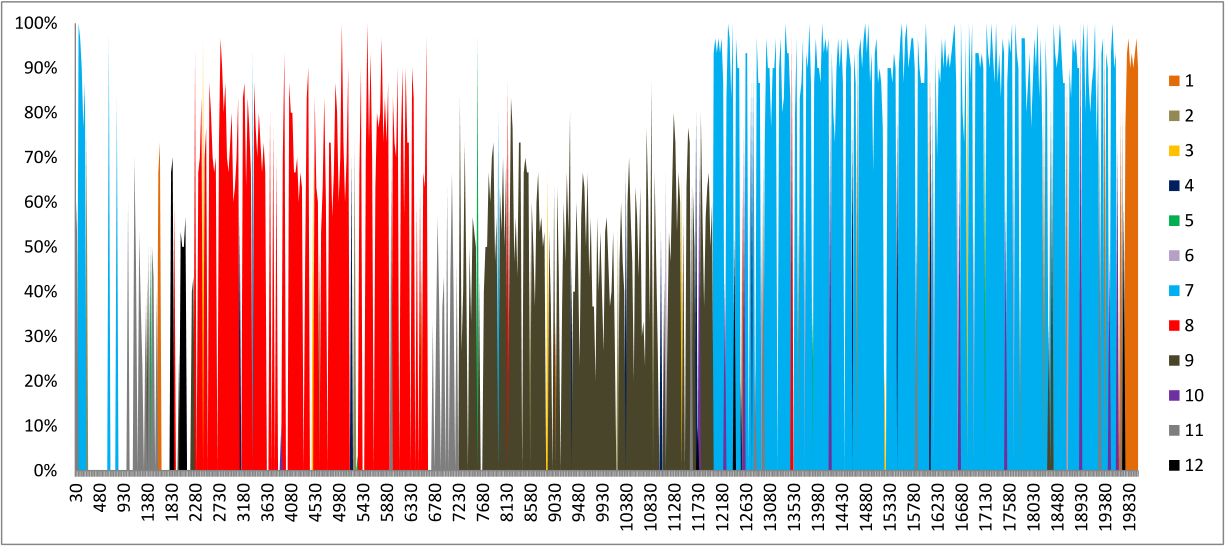
\includegraphics[width=.85\textwidth]{img/ql_exec_color.png}
	\caption{Varia��o de recebimento durante a execu��o do algoritmo QL}
	\label{fig:ql_exec}
\end{figure}

\begin{figure}[h]
	\center
	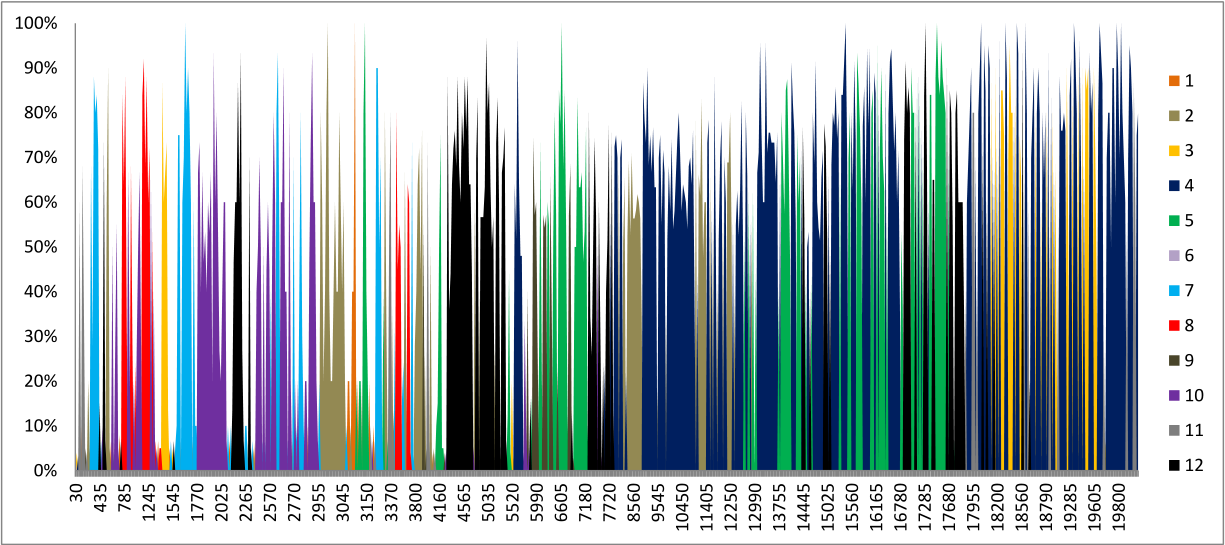
\includegraphics[width=.85\textwidth]{img/es_exec_color.png}
	\caption{Varia��o de recebimento durante a execu��o do algoritmo ES}
	\label{fig:es_exec}
\end{figure}

\section{Conclus�o}
\label{sec:conclusao}

Conclus�o

\bibliographystyle{sbc}
\bibliography{sbc-template}

\end{document}
